\clearpage

\section{Considerations}
The variety of available data is undeniable. 
Nevertheless, during the analysis, an issue emerged that is rarely 
addressed in the reviewed papers: the correctness of 
LLM-generated code. It is self-evident that anyone using 
LLM-generated code would, before committing it, 
most certainly run at least one test to verify that the 
code works. Moreover, for our purposes 
(\hyperref[sec:Motivations Behind LLM-Generated Code Detection]{Section 1.2}), 
whether a student or candidate submits non-functional 
code, it makes little difference whether it was written by them or 
by an LLM. 

A relevant concern arises from the lack of guarantee 
that the LLM-generated code present in the test datasets is 
correct. Another important question is whether there is a 
correlation between incorrect and correct code in the detection of 
LLM code. According to some analysed studies, the answer is affirmative: 
‘The results demonstrate that detecting correct code is more difficult 
than detecting incorrect code, both with our method and 
baselines.’~\cite{ye2023uncovering}

Therefore, the consideration that every detection method 
should be evaluated specifically on \textbf{functional} LLM-generated code, 
rather than on LLM code in general, proves useful in preventing a 
significant gap between the reported metrics and the actual user 
experience. Such a gap may arise if detection methods exhibit a 
classification bias due to the incorrect behaviour of the code. 
It is worth noting that while many works perform syntax or runtime 
checks, none explicitly mention functional testing.


\newpage
\subsection{Test framework}
\label{section:Test framework}
Given the evaluations presented by the works I propose, 
the detection methods, it was necessary to develop a framework that 
could ensure the LLM code was certainly correct. The minimum result was 
to obtain at least a subdataset that would allow evaluating whether there was a 
difference between detection of functioning and non-functioning code.

So a small framework was developed and published on
\href{https://github.com/DelGaudioNunzioSE/Code-LLMsTester.git}{GitHub}.
This framework had important constraints: 
\begin{itemize}
    \item It had to work with Python (the most generated programming language)
    \item It had to work on LLMs that could run on home hardware, 
    \item It had to support as many LLMs as possible, 
    \item It had to allow for the interruption and resumption 
of test generation and the tests themselves at any time, 
in order to evaluate error conditions and bugs.
\end{itemize}

\begin{figure}[H]
    \centering
    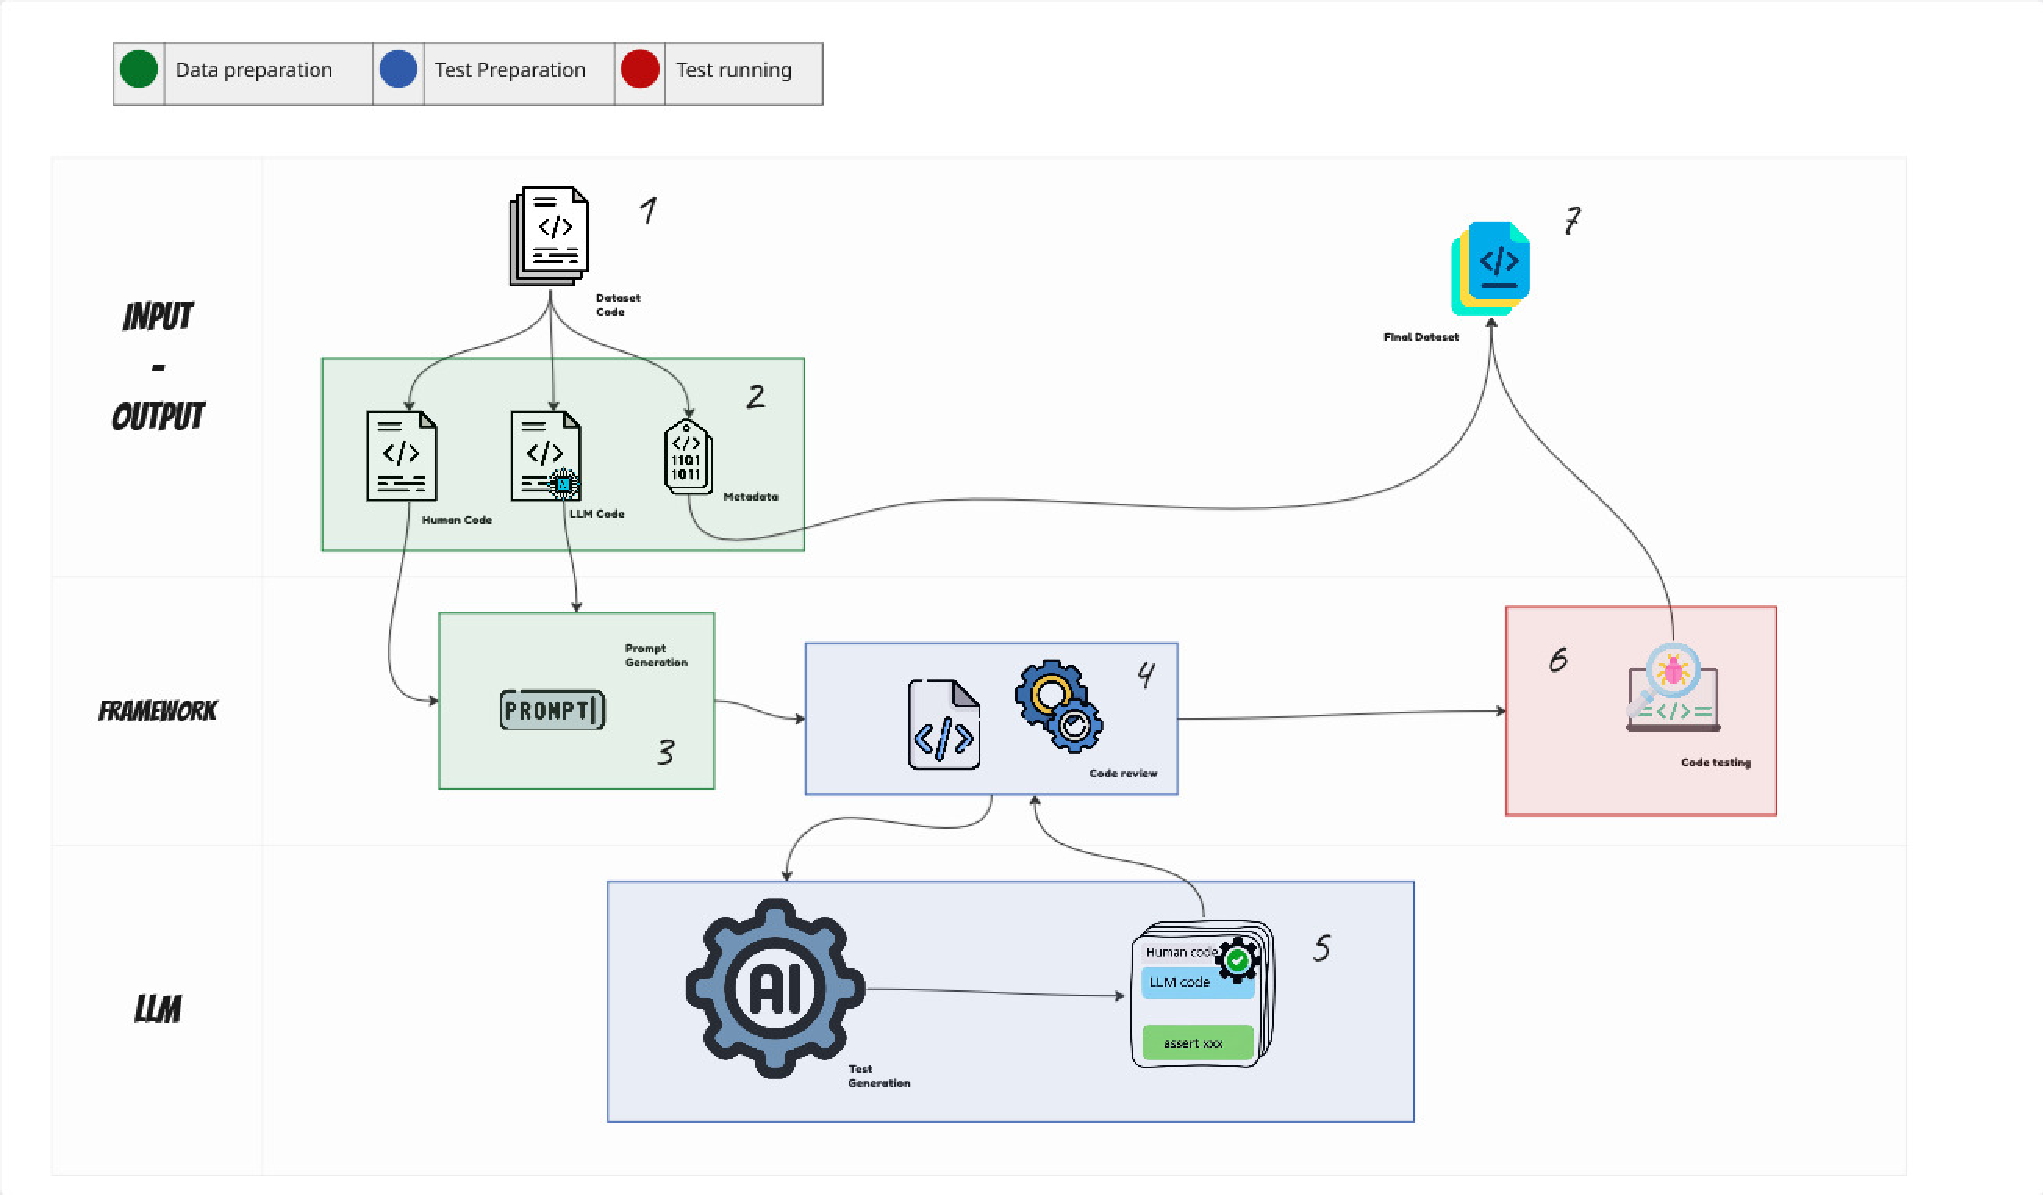
\includegraphics[width=1\textwidth]{img/framework/overview.pdf}
    \caption{Framework overview}
    \label{fig:framework overview}
\end{figure}


The framework was divided into several sections, so it could be easily modified for 
potential future needs that required dataset generation by an LLM.

\begin{enumerate}
\item \textbf{Input:}The framework is capable of processing any dataset 
that contains both LLM-generated code and human code that solve the same problem.

\item \textbf{Input\textbackslash Data preparatin:} Any supported dataset is converted into a JSON file, 
specifying which columns in the dataset correspond to \textit{"human code"} \textit{"LLM code"}, and 
\textit{“problem explanation”} (the latter being optional and included only to 
provide a more complete prompt to the LLM).

\item \textbf{Framework\textbackslash Data Preparation:} A prompt template has 
been prepared for an instruct-LLM. The prompt asks the LLM to understand both the LLM code and 
the human code that solve the same problem, with potentially different input formats. 
The model is asked to generate code that evaluates whether the two implementations return 
the same output values given the same input values (even if provided in different formats).



\item \textbf{Framework\textbackslash Test Preparation:} Since the LLMs used were "lightweight", 
both before passing the code to the LLM and after obtaining the final .py file, small 
adjustments are applied, such as: renaming classes and functions to ensure that the two 
solutions have different function and class names, adding missing imports 
(a common cause of test failures), and so on.

\item \textbf{LLM\textbackslash Test Preparation:} The LLM generates 3 inputs and 3 control assets in Python.

\item \textbf{Framework\textbackslash Test Running:} The framework therefore generates a folder 
to insert the test code, executes it, and collects the results, saving the number of tests 
passed for each code.

\item \textbf{Output:} The test results are collected and added to the 
metadata saved at the beginning of the process, with the aim of obtaining a 
final dataset containing information about the test execution.



\end{enumerate}




%%%%%%
\subsubsection{Development insights}
Firstly, it is important to underline a fundamental consideration:
the reason for not asking the LLM to directly classify the code as 
correct or incorrect is supported by the findings of the paper 
\textit{``Do LLMs generate test oracles that capture the actual or 
the expected program behaviour''}~\cite{konstantinou2024llms}, which states: 
\textit{``LLMs are more effective at generating test oracles rather than classifying them.''}

The framework has been developed starting from the project \textbf{KodCode}\cite{xu2025kodcode}, 
available on \href{https://github.com/KodCode-AI/kodcode/tree/main}{GitHub}. 
KodCode aims to generate code from prompts in order to train LLMs on 
synthetic code. 
However, the project underwent huge changes, leaving very 
little of the original code (like the \textit{.jsonl} use).


Initially, the idea was to slightly modify the \texttt{KodCode} 
framework so as not to require a large language model (LLM) 
to generate both code and tests, but only the tests. 
However, during the development and analysis of the 
framework, it became evident that much more substantial 
changes and additions were necessary.

First and foremost, it was necessary to develop a 
method for preprocessing and preparing a dataset of 
pre-written code. Subsequently, the entire generation 
phase had to be adapted to meet the new objectives.

After initial testing, it became clear that an LLM 
of moderate size (14B), a necessary compromise due to 
hardware limitations, was not sufficiently capable of 
understanding the problem and the code to generate 
effective tests. In many cases, the tests produced 
were incorrect and would have incorrectly flagged 
correct code as faulty.

As a result, it became necessary to change the approach: 
rather than relying solely on the LLM’s test-generation 
capabilities, functioning reference code that solved the 
same problem was used. Since the dataset proposed by 
Pan et al.\ includes both LLM-generated code and 
corresponding human-written code (the latter being reliably correct), 
the analysis concentrated on that dataset.

The new strategy required generating inputs consistent 
with both the problem statement and the function signatures. 
The LLM's task was thus limited to generating such inputs 
and writing code to verify whether both the human-written 
and LLM-generated implementations would produce the same 
outputs for those inputs.

Several challenges emerged from this new approach, some 
of which are outlined below:

\begin{enumerate}
    \item \textbf{Lack of Imports}: Human-written code in the 
    dataset did not include any imports. Therefore, a mechanism was 
    introduced to automatically insert the most common imports, as the 
    LLM proved ineffective at consistently adding all necessary ones.
    
    \item \textbf{Code Structure Variability}: Not all 
    solutions were simple functions—some were classes, 
    and others were standalone Python scripts. For class-based 
    solutions, the prompts were adapted to enable the LLM to 
    instantiate objects correctly and generate the necessary tests. 
    For script-based code, such examples were discarded, 
    since converting them into testable functions might have 
    introduced errors attributable to the transformation process 
    rather than to the code itself.
    
    \item \textbf{Name Collisions}: In many cases, 
    the human-written and LLM-generated code used identical 
    class or function names. To address this, an algorithmic 
    renaming strategy was implemented to avoid such conflicts.
\end{enumerate}

Subsequently, it became necessary to develop an 
entire sub-framework responsible for effectively 
generating the test files. These files needed to 
contain both the human-written and LLM-generated 
functions, as well as the tests produced by the LLM.

The sub-framework was also tasked with executing 
multiple tests in parallel, reporting the result of 
each individual execution, and generating a new dataset 
based on the previous one, but enriched with additional 
information regarding the outcome of the tests.

Despite the significant effort invested in 
developing the framework, it was decided to maintain, 
at least in this phase, certain limitations—potentially 
addressable in future work, such as compatibility with the 
Python programming language only.

%%%
\subsubsection{Possible improvements}
Despite the work done, there is still significant room for improvement:
\begin{itemize}
\item Predefined prompts depending on the LLMs
\item Support for APIs for test generation
\item Test execution within containers separate from the execution environment
\item Improvement of library import techniques
\end{itemize}